\documentclass[margin=2mm]{standalone}
%\usepackage{bm}
%\usepackage{calligra}
\usepackage{amsmath} % assumes amsmath package installed
\usepackage{amssymb}  % assumes amsmath package installed
\newcommand{\setfont}[2]{{\fontfamily{#1}\selectfont #2}}
\usepackage{graphicx}
\usepackage{tikz}
\usetikzlibrary{3d}

\usetikzlibrary{calc}
\usetikzlibrary{patterns}
\usetikzlibrary{decorations.text}
\usetikzlibrary{decorations.pathmorphing}
\usetikzlibrary{decorations.markings}
\usetikzlibrary{arrows}
\usetikzlibrary{shapes}

%\pgfdeclareimage[width=2.0cm]{VectorFields}{EllipseBetaThird}
%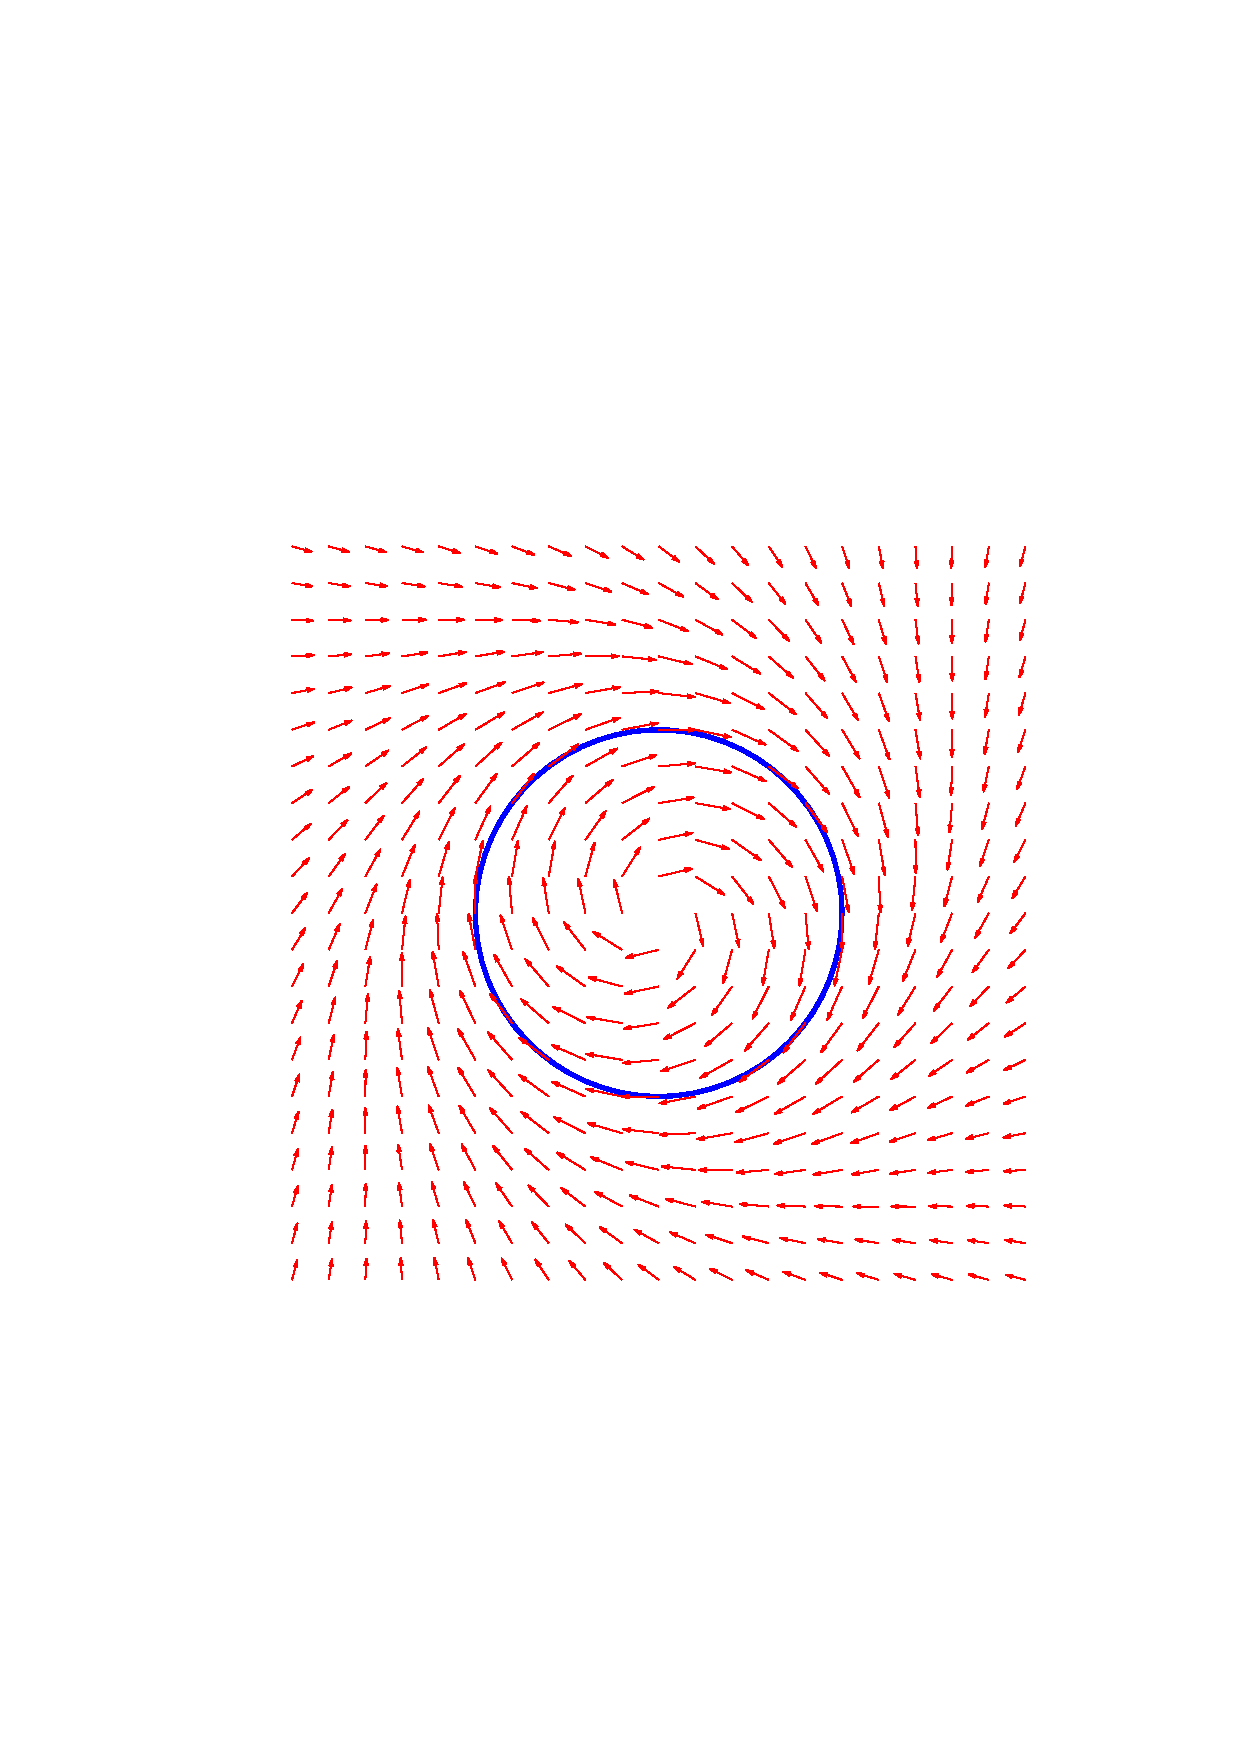
\includegraphics[trim=4cm 10cm 4cm 11cm, clip=true,keepaspectratio,width=0.45\linewidth]{../Fig3a_UnitCircle.pdf}

\newcommand{\picturefontsize}{\LARGE}
\newcommand{\pictureLineWidth}{0.8mm}

\begin{document}
% For every picture that defines or uses external nodes, you'll have to
% apply the 'remember picture' style. To avoid some typing, we'll apply
% the style to all pictures.
\tikzstyle{every picture}+=[remember picture]
\tikzstyle{na} = [baseline=-.5ex]

\begin{tikzpicture}

%\draw[help lines,thick] (-2,-4) grid (7,2);

\tikzstyle{vflabels}=[font=\tiny];
% First Line: Images

\node (imagea) at (0,0)
{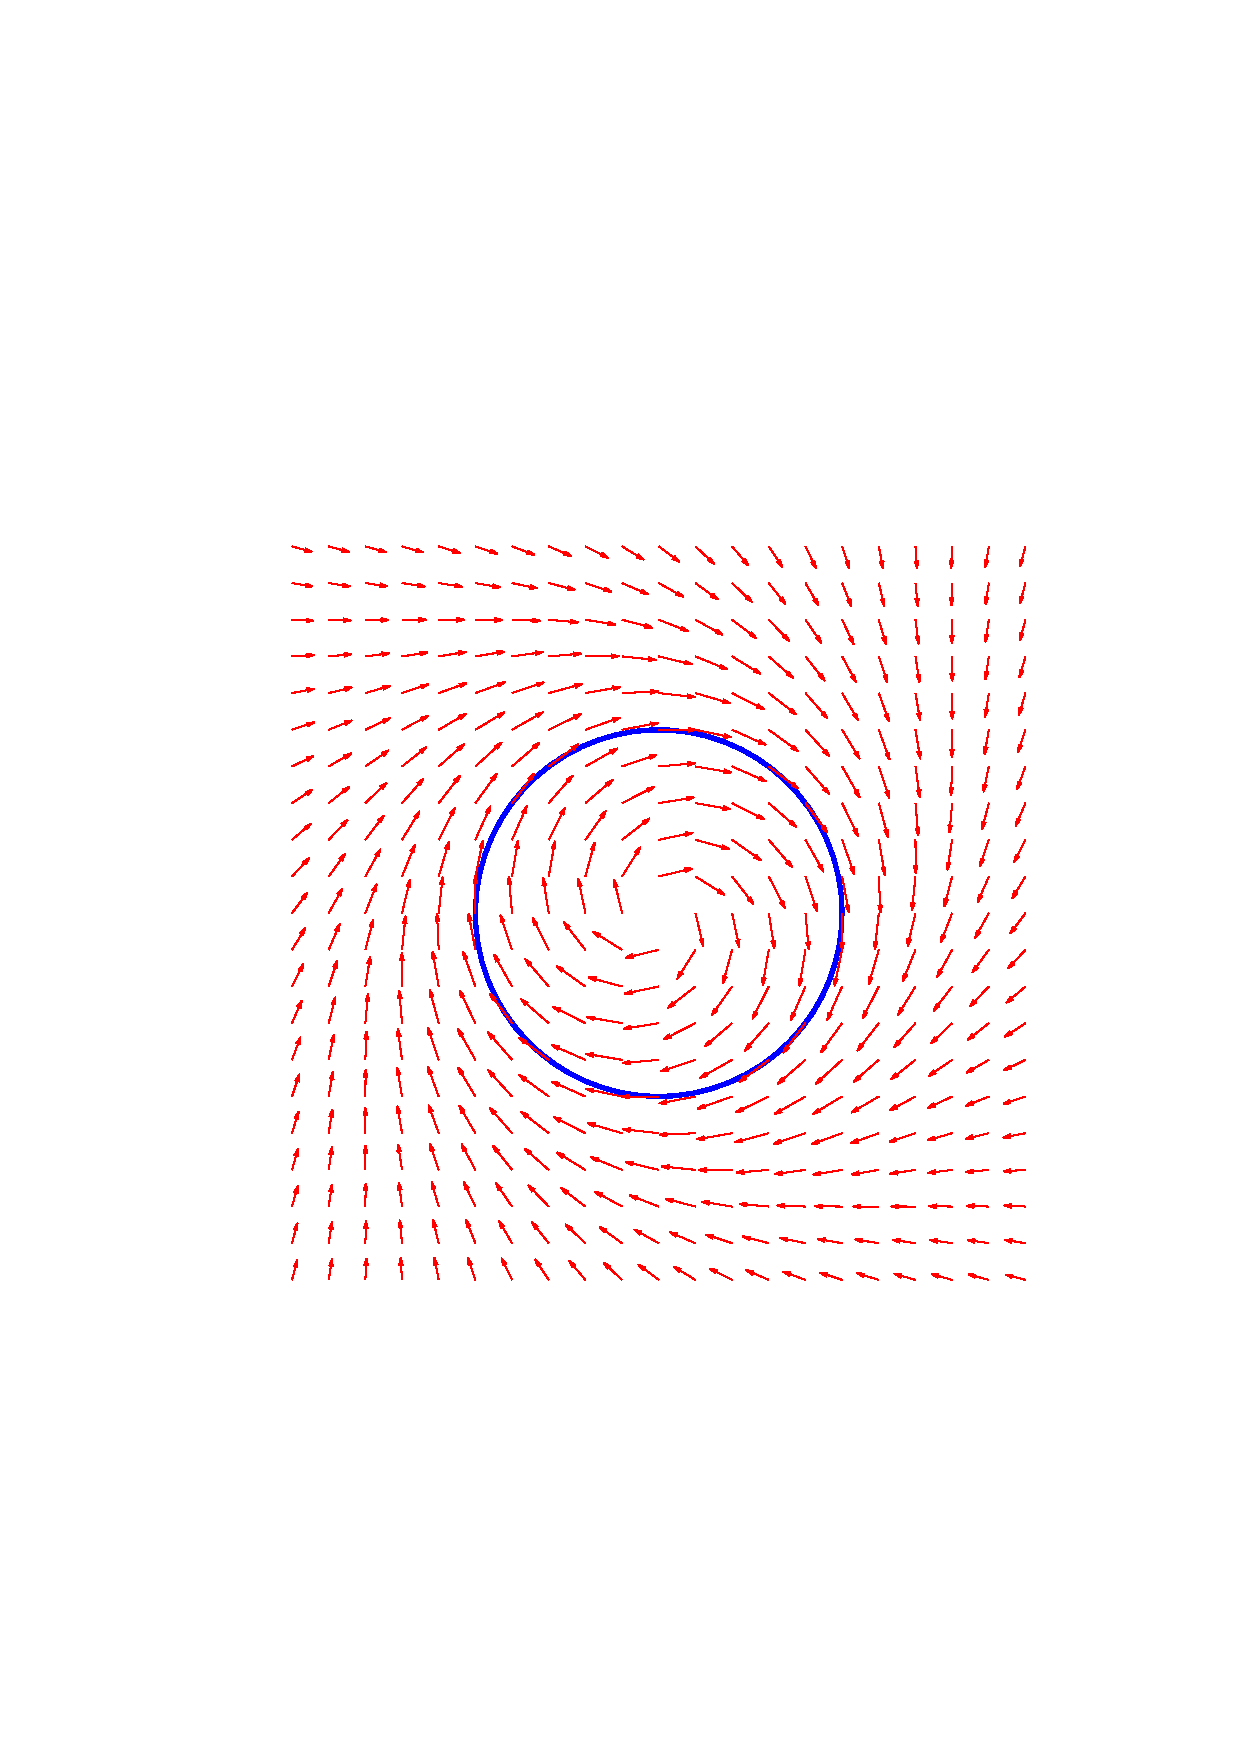
\includegraphics[trim=4cm 10cm 4cm 11cm, clip=true,keepaspectratio,width=2cm]{../Fig3a_UnitCircle.pdf}}; 
\node[vflabels] at (0,-0.8) (labelimagea) {(a)};

\node (imageb) at (2.5,0.0)
{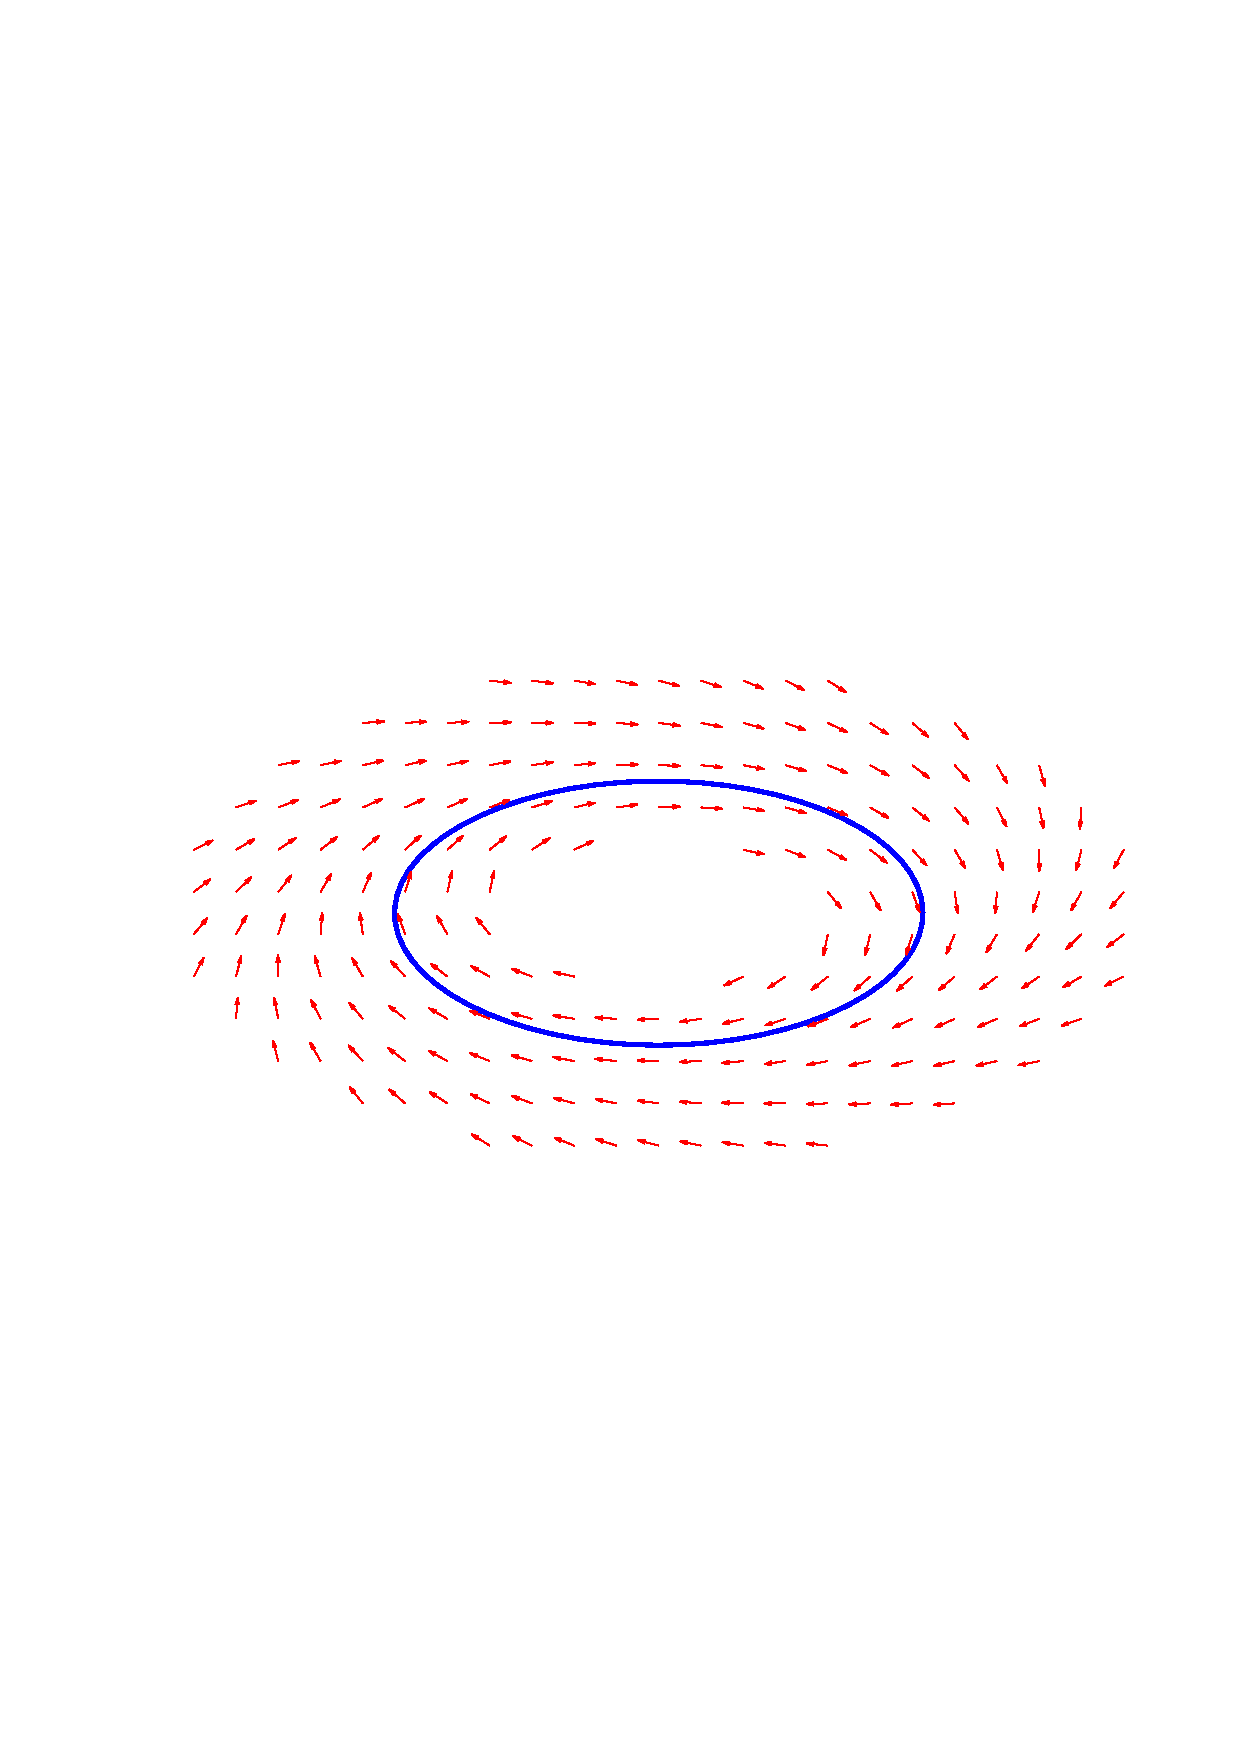
\includegraphics[trim=2.5cm 9cm 1cm 10cm, clip=true,keepaspectratio,width=2cm]{../Fig3b_Ellipse.pdf}}; 
\node[vflabels] at (2.5,-0.8) (labelimageb) {(b)}; 

% Third line: Images
\node (imagec) at (0,-1.6)
{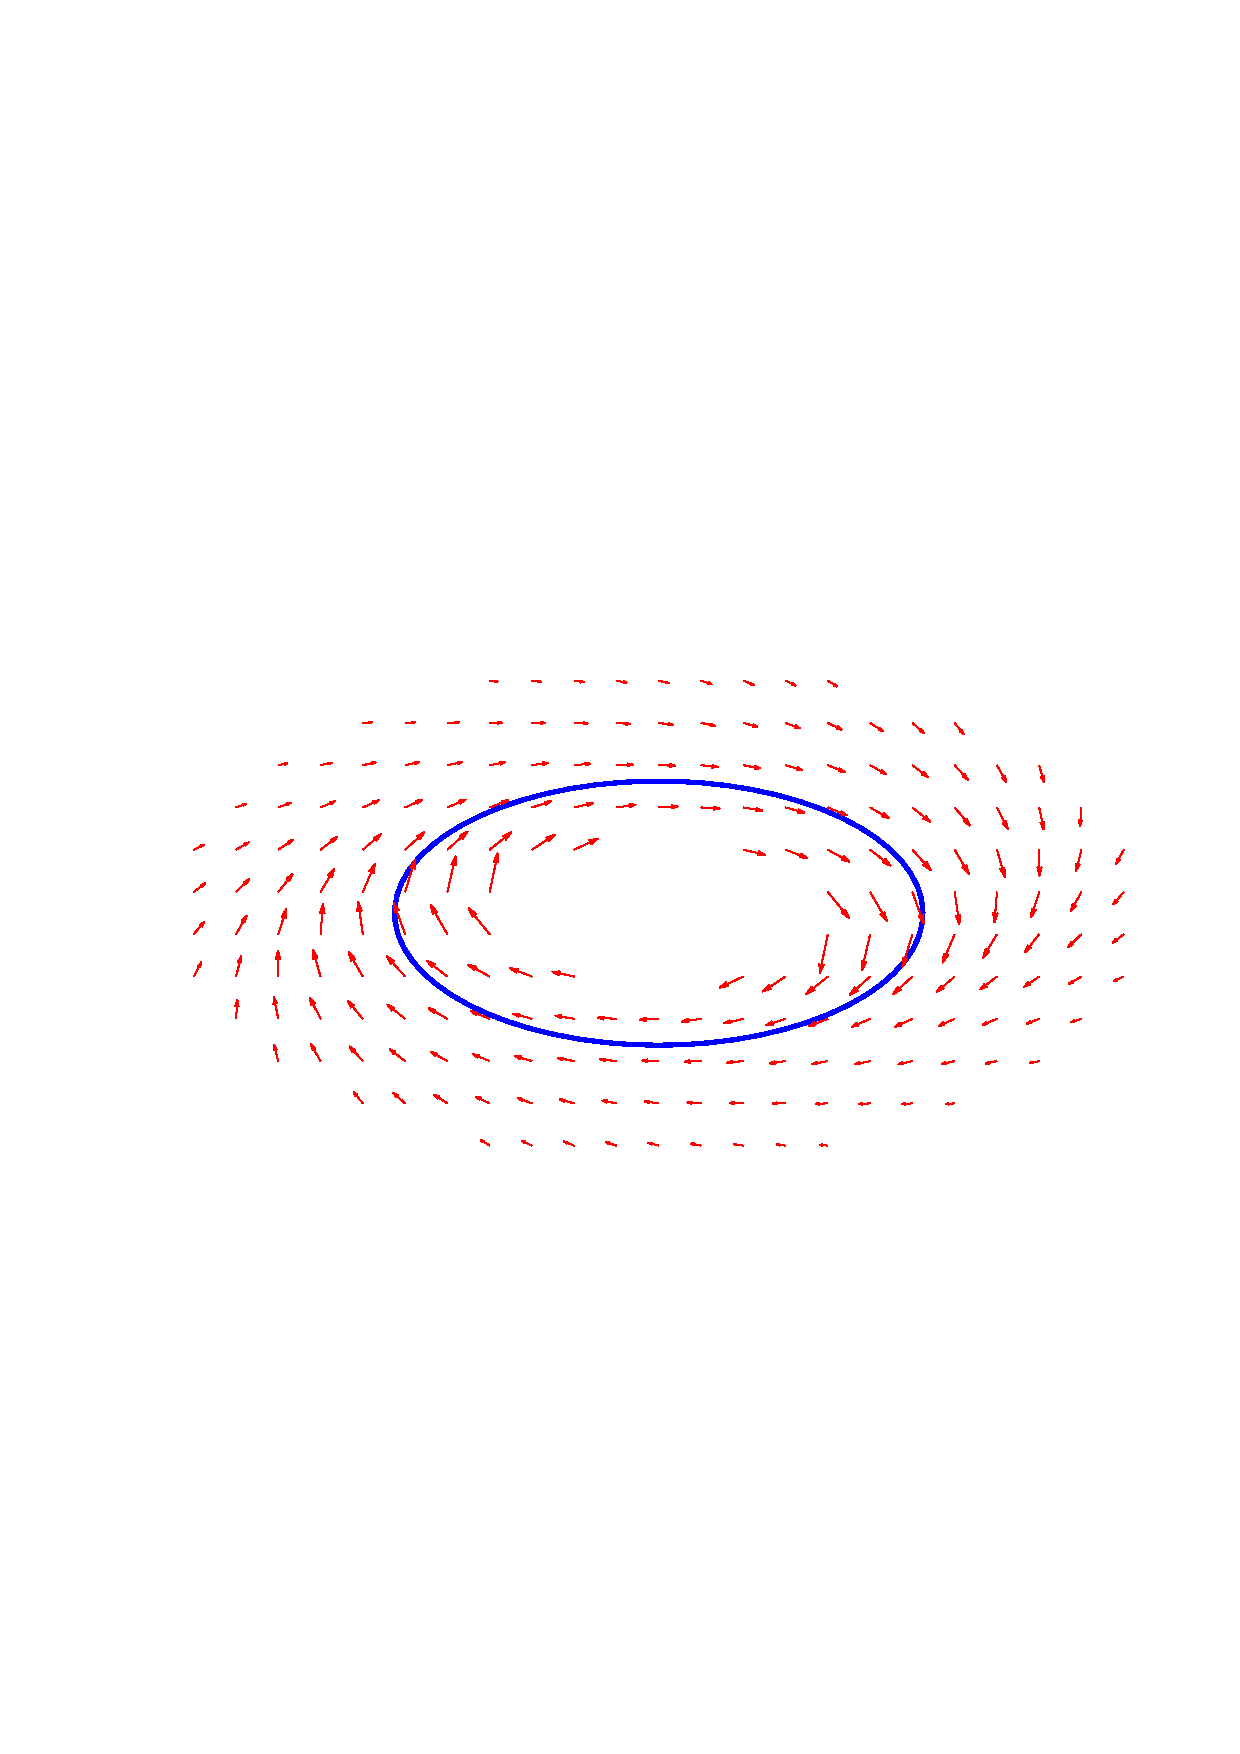
\includegraphics[trim=3cm 9cm 1cm 10cm, clip=true,keepaspectratio,width=2cm]{../Fig3c_EllipseBetaMinusThird.pdf}}; 
\node[vflabels] (labelimagec) at (0,-2.3) {(c)};

\node (imaged) at (2.5,-1.6)
{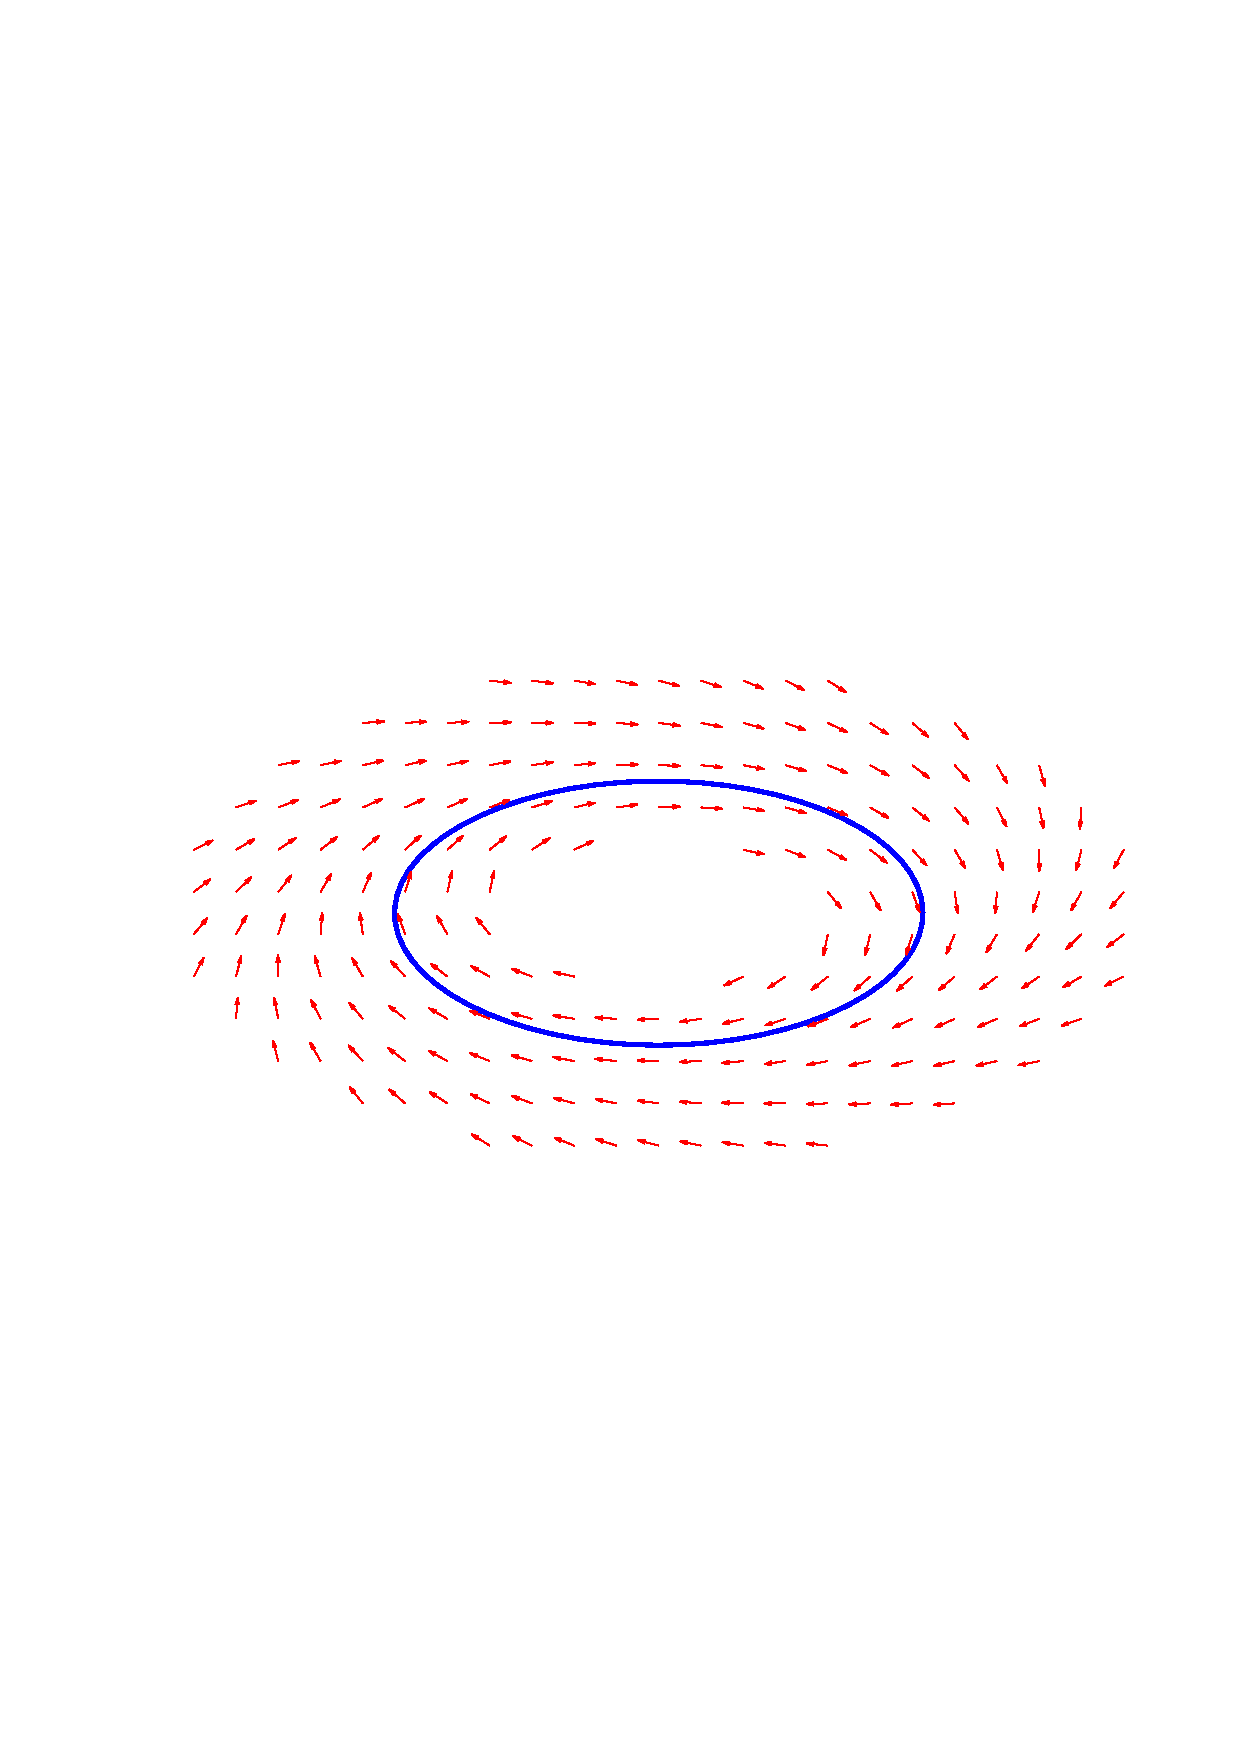
\includegraphics[trim=3cm 9cm 1cm 10cm, clip=true,keepaspectratio,width=2cm]{../Fig3d_EllipseBetaZero.pdf}}; 
\node[vflabels] (labelimaged) at (2.5,-2.3)  {(d)}; 
% Fourth line: labels

% Fifth line: images
\node (imagee) at (0,-3)
{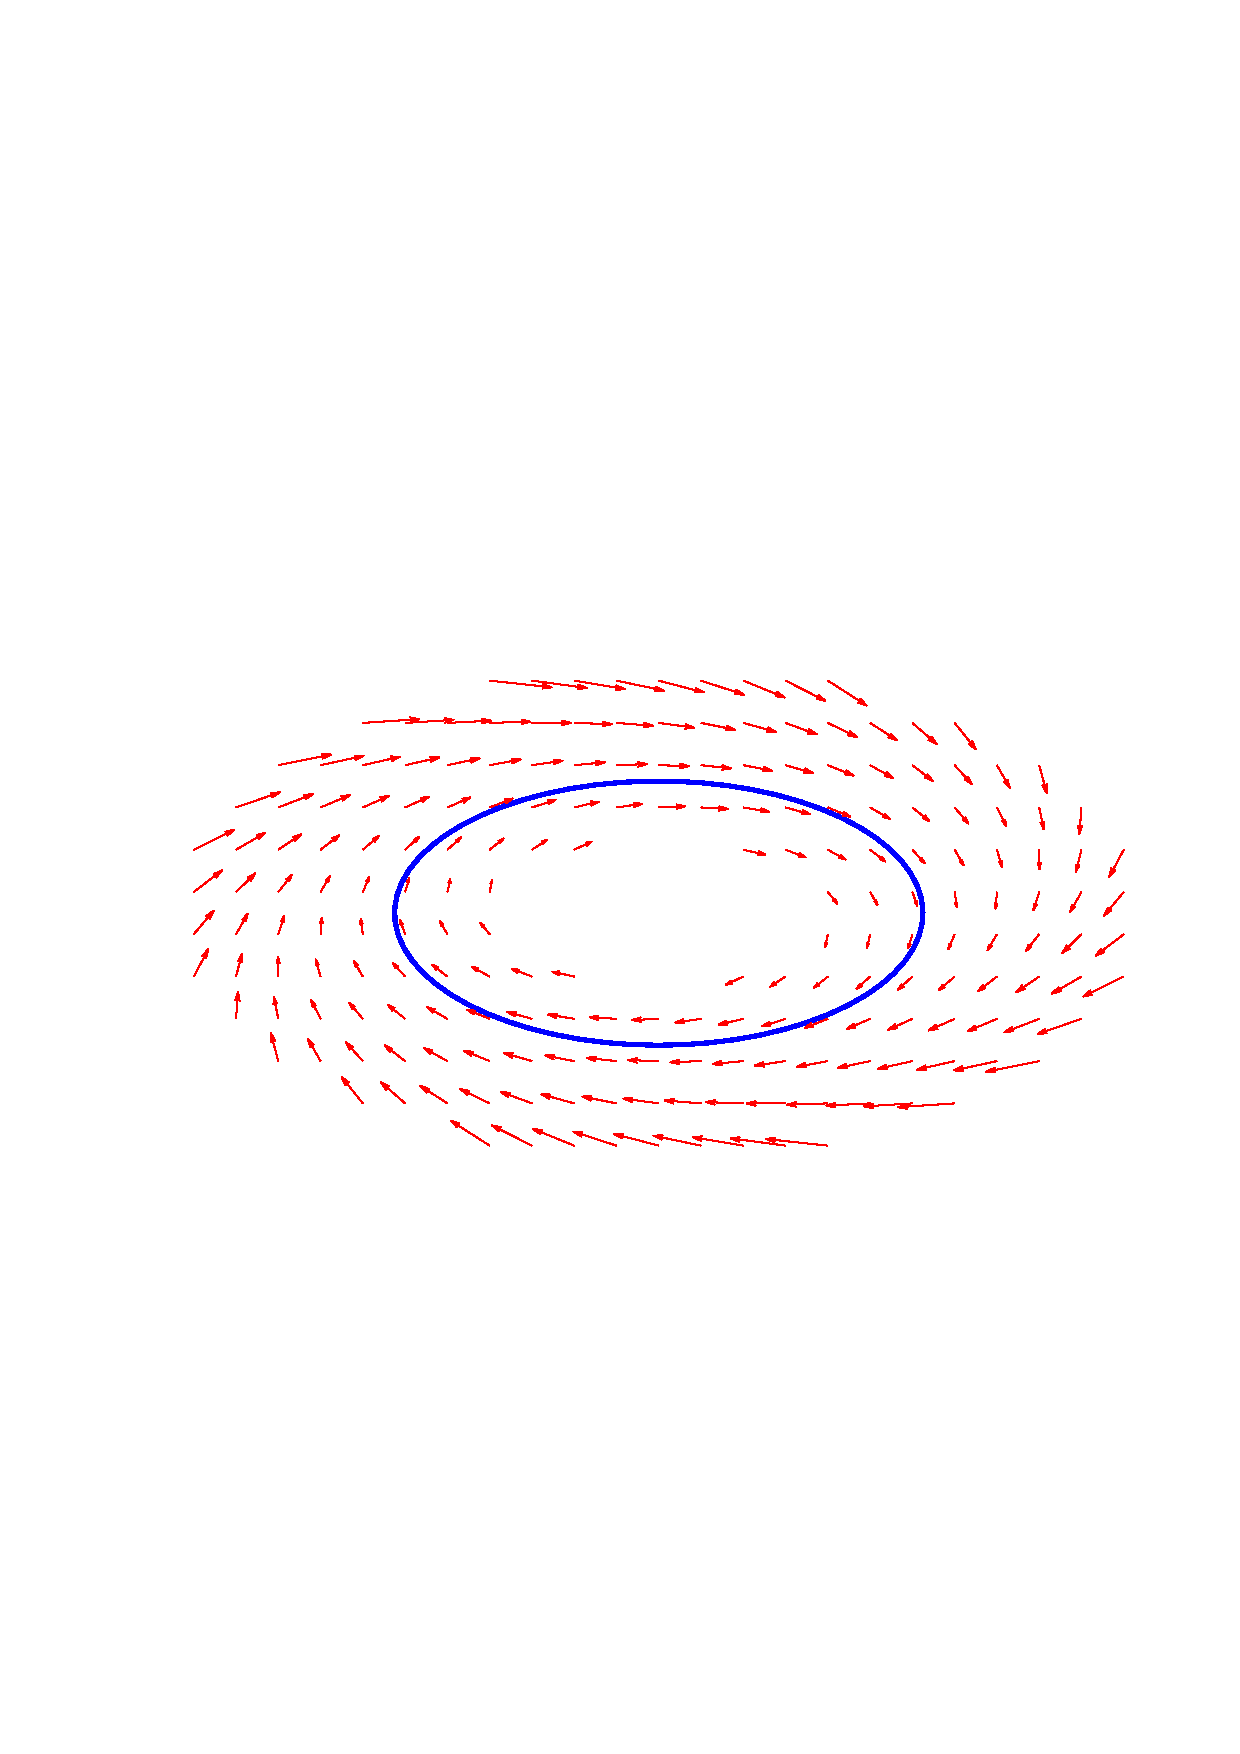
\includegraphics[trim=3cm 9cm 1cm 10cm, clip=true,keepaspectratio,width=2cm]{../Fig3e_EllipseBetaThird.pdf}}; 
\node[vflabels] (labelimagee) at (0.,-3.7)  {(e)};

\node (imagef) at (2.5,-3)
{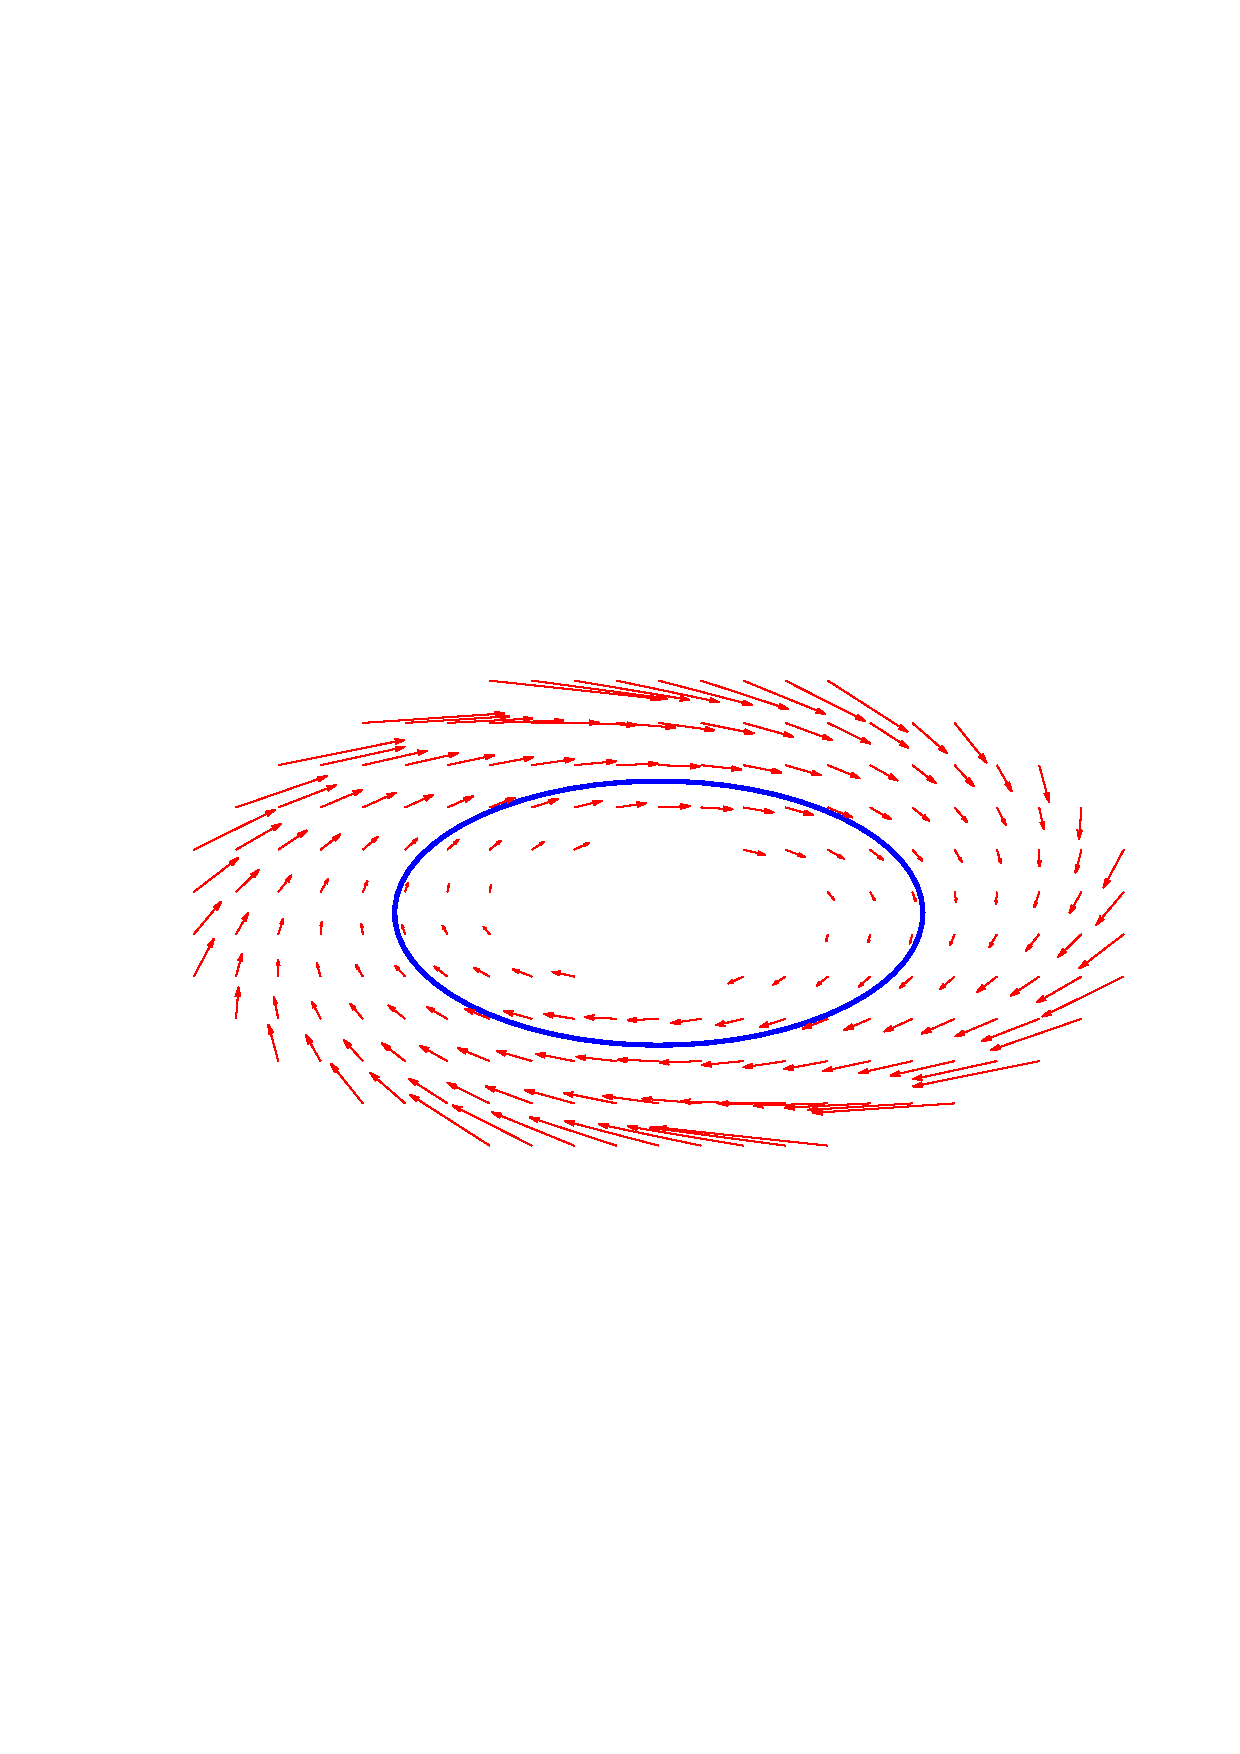
\includegraphics[trim=3cm 9cm 1cm 10cm, clip=true,keepaspectratio,width=2cm]{../Fig3f_EllipseBetaTwoThirds.pdf}}; \\
% Sith line: labels
\node[vflabels] (labelimagef) at (2.5,-3.7) {(f)};

%\node (zero) at (0,0) {$(0,0)$};
\end{tikzpicture}
\end{document}
